% шрифт
\documentclass[]{article}
\usepackage[english,russian]{babel} 
\usepackage{fontspec} 
\defaultfontfeatures{Ligatures={TeX}} 
\setmainfont{PT Astra Serif}
%\renewcommand\normalsize{\fontsize{14}{16.8pt}\selectfont}
\renewcommand\normalsize{\fontsize{14}{21pt}\selectfont}
%\setmainfont[Ligatures={TeX,Historic}]{PT Astra Serif}

% размер страницы
\usepackage[a4paper, left=2.5cm, right=1.5cm, top=2.5cm, bottom=2.5cm]{geometry}

% формулы
\usepackage{amsmath}
\usepackage{amssymb}
%\renewcommand\leq{\leqslant}
%\renewcommand\geq{\geqslant}
% перенос формул в тексте
%\newcommand*{\hm}[1]{#1\nobreak\discretionary{}%
%	{\hbox{\mathsurround=0pt \ensuremath{#1}}}{}}

% рисунки
\usepackage{graphicx}
\usepackage{xcolor}

% таблицы
%\usepackage{ctable}% http://ctan.org/pkg/ctable
\usepackage{caption}% http://ctan.org/pkg/caption

% абзац
\usepackage{indentfirst}	% отступ первой строки
%\setlength\parindent{15mm}	% отступ

% перечисления
%\setlength{\listparindent}{1.5em}%   Красная строка
\usepackage{enumitem}
\setlist[enumerate,itemize]{leftmargin=0pt,itemindent=1.0em,listparindent=1.0em}
%\setlist[enumerate,itemize]{leftmargin=10pt,itemindent=2.7em,rightmargin=2cm,listparindent=1.5em}

% нумерация библиографии
\makeatletter
\def\@biblabel#1{#1. }

\makeatother

%\usepackage{blindtext}

%opening
\title{\Large{Вариант реализации конечноэлементного решения упругопластической задачи при наличии контакта с жёстким штампом}}
\author{}
\date{}
%\date{\today}

\begin{document}
\maketitle
\begin{abstract}
\large{Рассматривается квазистатическая задача контакта изотропного, упругопластического, изотропно упрочняющегося тела и жёсткого штампа без трения для случая малых деформаций. Поведение материала определяется теорией пластического течения с условием текучести Мизеса и диаграммой одноосного растяжения, в качестве параметра упрочнения принимается параметр Одквиста. В этой работе приведён алгоритм шагового конечноэлементного решения данной задачи, совмещающий метод начальных напряжений с построением касательной матрицы жёсткости, которая преимущественно остаётся неизменной при итерациях. Условия контакта удовлетворяются расширенным методом множителей Лагранжа, который приводит к отсутствию зазора между узлами сетки и штампом. На примере вдавливания жёсткого шара в упругопластичное полупространство со степенным упрочнением, в трёхмерной постановке, показана работоспособность реализации алгоритма.}
\end{abstract}

\section{Введение}
Применение универсальных средств расчёта напряжённо-деформированного состояния, таких как ANSYS, в отдельных случаях может быть осложнено большими вычислительными затратами или некоторыми проблемами с определением требуемых видов нелинейностей или со сходимостью итераций. Это обстоятельство обуславливает потребность в построении узкоспециализированных вычислительных средств. В качестве базовой рассматривается задача контакта упругопластичного тела с жёстким подвижным штампом.

Наиболее распространённым методом решения нелинейных задач является метод Ньютона-Рафсона \cite{Bathe1982}, признанный наиболее быстро сходящимся в вычислительной практике и является основным в большинстве современных средств расчёта, но он требует обновления матрицы жёсткости на каждой итерации, а модифицированный метод Ньютона-Рафсона требует большого количества итераций. В данной работе физическая нелинейность учитывается совмещением построения касательной матрицы жёсткости и метода начальных напряжений \cite{Zienkiewicz1975}: в начале шага по времени матрица строится по начальному приближению и меняется на итерациях только когда прогнозируется разгрузка после активного нагружения; величины пластических деформаций корректируются радиальным возвратом на поверхность текучести.

Среди алгоритмов учёта контакта \cite{Burago2005} выделяется метод множителей Лагранжа, точно обеспечивающий условие непроникания, но его реализация требует введения дополнительных степеней свободы в СЛАУ (множителей Лагранжа), что замедляет итерации и усложняет реализацию. Поэтому для учёта контакта мы реализовали расширенный метод Лагранжа \cite{Wriggers2006}, основанный на многократном применении метода штрафа и позволяющий регулировать соотношение скорости сходимости к увеличению обусловленности СЛАУ, которое происходит из-за добавления контактных жёсткостей в матрицу.

\section{Постановка задачи}
В области $\Omega$ заданы уравнения равновесия \cite{Pisarenko1981}
\begin{equation}
%\sum\limits_{j=1}^{3} \frac{\partial\sigma_{ij}}{\partial x_j} = 0, i=\overline{1,3}.
%\frac{\partial\sigma_{ij}}{\partial x_j} = 0, i=\overline{1,3}.
%\bigtriangledown_j\sigma_{ij} = 0.%, i=\overline{1,3}.
\frac{\partial\sigma_{ij}}{\partial x_j} = 0.%, i=\overline{1,3}.
\label{F:F1}
\end{equation}
На границе $S=S_{1}\cup S_{2}$ заданы кинематические и силовые
краевые условия
\begin{equation}
\left.\mathbf{u}\right|_{S_{1}}=\mathbf{u}_{0}\left(t\right),
\label{F:F2}
\end{equation}
\begin{equation}
%\left.\sum\limits_{j=1}^{3}\sigma_{ij}n_j\right|_{S_{2}}=P_{i}\left(t\right),\:i=\overline{1,3},
\left.\sigma_{ij}n_j\right|_{S_{2}}=P_{i}\left(t,\,\mathbf{u}\right),% i=\overline{1,3},
\label{F:F3}
\end{equation}
\begin{equation}
\mathbf{P}\left(t,\,\mathbf{u}\right)=\mathbf{P}^t\left(t\right)+\mathbf{P}^c\left(t,\,\mathbf{u}\right),
\label{F:F_Contact_razlojenie}
\end{equation}
где $\mathbf{u}$ --- вектор перемещения, $\mathbf{n}$ --- внешняя единичная нормаль к поверхности $S_{2}$, $\mathbf{P}$ --- вектор поверхностных сил, $\mathbf{P}^t$ --- составляющая внешнего силового воздействия, $\mathbf{P}^c$ --- контактная составляющая на $S_c\subseteq S_2$.

На границе $S_{c}$ задаётся механический контакт с жёстким подвижным штампом геометрически нелинейными краевыми условиями Синьорини \cite{Kravchuk1994} 
\begin{equation}
\begin{cases}
\mathbf{P}^c\cdot\mathbf{n}\leq 0, \\
\mathbf{u}\cdot\mathbf{n}-g\leq 0, \\
\left(\mathbf{P}^c\cdot\mathbf{n}\right) \left(\mathbf{u}\cdot\mathbf{n}-g\right)=0, \\
\left( \mathbf{P}^c\cdot\mathbf{n}\right)\mathbf{n}=\mathbf{P}^c, \\
\end{cases}
\label{F:F_Contact_Signorini}
\end{equation}
где $\mathbf{n}\left(\mathbf{x},\,\mathbf{t}\right)$ --- внутренняя единичная нормаль в точке поверхности штампа, ближайшей к точке тела $\mathbf{x}$, $g\left(\mathbf{x},\,\mathbf{t}\right) $ --- расстояние от точки $\mathbf{x}$ до поверхности штампа (может принимать отрицательные значения в случае внедрения штампа).


Компоненты тензора малых деформаций Коши $\varepsilon$ связаны с перемещениями линейными геометрическими соотношениями
\begin{equation}
\varepsilon_{ij}=\frac{1}{2} \left(\frac{\partial u_{i}}{\partial x_{j}} + \frac{\partial u_{j}}{\partial x_{i}} \right).
\label{F:F4}
\end{equation}

Для изотропного тела тензор напряжений Коши $\sigma$ выражается через упругую составляющую $\varepsilon^{e}$ малой деформации Коши обобщенным законом Гука
\begin{equation}
%\sigma_{ij}=\sum\limits_{l=1}^{3} \sum\limits_{k=1}^{3} C_{ijkl}\varepsilon_{kl}^{e},
%\sigma_{ij}=C_{ijkl}\varepsilon_{kl}^{e},
\sigma=C:\varepsilon^{e},
\label{F:F_Hook}
\end{equation}
\begin{equation}
C_{ijkl}=\lambda\delta_{ij}\delta_{kl}+\mu\left(\delta_{ik}\delta_{jl}+\delta_{il}\delta_{jk}\right),
\label{F:F5}
\end{equation}
где $C$ --- тензор модулей упругости материала, $\lambda$, $\mu$ --- модули упругости Ламэ, $\delta$ --- символ Кронекера. Символом \textquotedblleft $:$\textquotedblright обозначено двойное скалярное произведение, т.е. $\left(C:\varepsilon\right)_{ij}\equiv C_{ijkl}\varepsilon_{kl}$.

Для связи напряжений и деформаций принимаются определяющие соотношения теории пластического течения \cite{Korobeynikov2000} с критерием текучести Мизеса:
\begin{equation}
d\varepsilon=d\varepsilon^{e} + d\varepsilon^{p},
\label{F:F_Flow1}
\end{equation}
\begin{equation}
\sigma_{y}=\Phi\left(q\right),
\label{F:F_Flow2}
\end{equation}
\begin{equation}
\begin{cases}
d\varepsilon_{ij}^{p}=\frac{\partial\tilde{\sigma}}{\partial\sigma_{ij}}d\lambda=\frac{\frac{3}{2}s_{ij}}{\tilde{\sigma}} d\lambda, \mbox{ если } \tilde{\sigma}=\sigma_{y} \mbox{ и } dW>0, \\
d\varepsilon_{ij}^{p}=0, \mbox{ если } \tilde{\sigma}<\sigma_{y} \mbox{ или } \tilde{\sigma}=\sigma_{y} \mbox{ и } dW\leq 0,
\end{cases}
\label{F:F_Flow3}
\end{equation}
где $d\lambda$ --- не известный множитель,
\begin{equation}
d\lambda=d\tilde{\varepsilon}^{p},
\label{F:F_FlowDef1}
\end{equation}
$\sigma_{y}$ --- предел текучести, $\Phi\left(q\right)$ --- функция, характеризующая поведение изотропно упрочняющегося материала (функцию $\Phi\left(q\right)$ можно построить по диаграмме одноосного растяжения, при котором $\tilde{\sigma}=\sigma$, $d\tilde{\varepsilon}^{p}=d\varepsilon^{p}$),
$d\varepsilon$, $d\varepsilon^{e}$, $d\varepsilon^{p}$ --- приращения полной, упругой и пластической деформаций соответственно, $\tilde{\sigma}\equiv\left(\frac{3}{2}s_{ij}s_{ij}\right)^{\frac{1}{2}}$ --- эквивалентное напряжение, $\tilde{\varepsilon}\equiv \left(\frac{2}{3}e_{ij}e_{ij}\right)^{\frac{1}{2}}$ --- эквивалентная деформация, $s_{ij}\equiv\sigma_{ij}-\delta_{ij}\frac{1}{3}\sigma_{kk}$ --- девиатор напряжений, $e_{ij}\equiv\varepsilon_{ij}-\delta_{ij}\frac{1}{3}\varepsilon_{kk}$ --- девиатор деформаций, $q$ --- параметр Одквиста,
\begin{equation}
q\equiv\int d\tilde{\varepsilon}^{p},
\label{F:F_FlowDef6}
\end{equation}
$dW$ --- девиаторная работа приращения деформаций,
\begin{equation}
dW\equiv s_{ij}d\varepsilon_{ij}.
\label{F:F_FlowDef7}
\end{equation}


\section{Дискретизация}
Домножим уравнения \eqref{F:F1} на пробную функцию $\upsilon$, применим формулу Грина интегрирования по частям и учтём силовые краевые условия \eqref{F:F3}, в результате система вариационных уравнений в форме Галеркина примет вид \cite{SoloveychikRoyakPersova2007}
\begin{equation}
\int\limits_{\Omega}\sigma_{ij}\frac{\partial\upsilon}{\partial x_j}  d\Omega=\int\limits_{S_{2}}P_{i} \upsilon dS.
\label{F:F_var2}
\end{equation}

Согласно шаговому методу для случая малых деформаций \cite{Zienkiewicz1975,Frolov1995}, для некоторого шага по времени $t\longrightarrow t+\Delta t$ запишем уравнение \eqref{F:F_var2} в приращениях

\begin{equation}
\int\limits_{\Omega}\Delta\sigma_{ij}\frac{\partial\upsilon}{\partial x_j} d\Omega=\int\limits_{S_{2}}\Delta P_{i} \upsilon dS + R_{i},
\label{F:F_var3}
\end{equation}
\begin{equation}
R_{i} \equiv \int\limits_{S_{2}}{}^{(t)}P_{i} \upsilon dS - \int\limits_{\Omega}{}^{(t)}\sigma_{ij}\frac{\partial\upsilon}{\partial x_j} d\Omega,
\label{F:F_var3_add}
\end{equation}
где $R_{i}$ имеет смысл невязки между внутренними напряжениями и силовыми воздействиями, которая понадобится для численной реализации. Здесь и далее для переменных по умолчанию подразумевается момент времени $t+\Delta t$, а момент времени $t$ обозначается левым верхним индексом $(t)$; для областей и границ всегда подразумевается момент времени $t$ и обозначение времени опущено.

Запишем закон Гука \eqref{F:F_Hook} с учётом \eqref{F:F_Flow1} в приращениях
\begin{equation}
\Delta\sigma=C:\left(\Delta\varepsilon-\Delta\varepsilon^{p}\right).
\label{F:F_alg_ce1}
\end{equation}
С целью последующей численной реализации, совмещающей построение касательной матрицы жёсткости и метода начальных напряжений, одну часть приращения $\Delta\varepsilon^{p}$ учтём путём изменения тензора модулей упругости $C$ на упругопластический тензор $\tilde{C}$, другую часть --- путём добавления начальных напряжений $\Delta\sigma^{0}$, то есть запишем определяющие соотношения в виде
\begin{equation}
\Delta\sigma=\tilde{C}:\Delta\varepsilon+\Delta\sigma^{0},
\label{F:F_alg_ce_main}
\end{equation}
где
\begin{equation}
\Delta\varepsilon^{p}=\Delta\varepsilon^{\tilde {C}}+\Delta\varepsilon^{\Delta\sigma^{0}},
\label{F:F_alg_ce2}
\end{equation}
\begin{equation}
\Delta\sigma^{0}=-C:\Delta\varepsilon^{\Delta\sigma^{0}},
\label{F:F_alg_ce3}
\end{equation}
\begin{equation}
\tilde{C}:\Delta\varepsilon=C:\left(\Delta\varepsilon-\Delta\varepsilon^{\tilde{C}}\right).
\label{F:F_alg_ce4}
\end{equation}
Для нахождения $\tilde{C}$, с учётом закона течения \eqref{F:F_Flow3} составим систему
\begin{equation}
\begin{cases}
\Delta\sigma^{\tilde{C}}=C:\left(\Delta\varepsilon-\Delta\varepsilon^{\tilde{C}}\right)\\
z:\Delta\sigma^{\tilde{C}}=\Delta\tilde{\sigma}^{\tilde{C}}\\
\Delta\varepsilon^{\tilde{C}}=z \Delta\tilde{\varepsilon}^{\tilde{C}}\\
\Delta\tilde{\sigma}^{\tilde{C}}=E^{*}\Delta\tilde{\varepsilon}^{\tilde{C}},
\end{cases}
\label{F:F_alg_ce_system}
\end{equation}
где
\begin{equation}
z_{ij}\equiv\frac{\partial{}^{(t)}\tilde{\sigma}}{\partial\sigma_{ij}}=\frac{\frac{3}{2}{}^{(t)}s_{ij}}{{}^{(t)}\tilde{\sigma}},
\label{F:F_alg_ce10}
\end{equation}
$E^{*}=\frac{\Delta\tilde{\sigma}^{\tilde{C}}}{\Delta\tilde{\varepsilon}^{\tilde{C}}}$ --- параметр упрочнения. При $\tilde{\sigma}\neq 0$, из \eqref{F:F_alg_ce_system} следует известное \cite{Zienkiewicz1975,Belytschko2000} выражение
\begin{equation}
\begin{gathered}
\tilde{C}=C-\frac{\left(C:z\right)\otimes \left(z:C\right) }{E^{*}+z:\left(C:z\right)},
\label{F:F_alg_C_pl}
\end{gathered}
\end{equation}
где символом \textquotedblleft $\otimes$\textquotedblright \ обозначено тензорное произведение, т.е. $\left( a\otimes b\right)_{ijkl} \equiv a_{ij}b_{kl}$.
Используя \eqref{F:F5}, можно упростить выражение компонент $\tilde{C}$
\begin{equation}
\begin{gathered}
\tilde{C}_{ijkl}=C_{ijkl}-\frac{4\mu^2}{E^{*}+3\mu}z_{ij}z_{kl}.
\label{F:F_alg_C_pl_parts}
\end{gathered}
\end{equation}

С учётом \eqref{F:F_alg_ce3}, составляющие приращения $\Delta\varepsilon^{p}$
\begin{equation}
\Delta\varepsilon^{\tilde{C}}=\left(\frac{2\mu}{E^{*}+3\mu}z\otimes z\right):\Delta\varepsilon=2\mu\frac{z:\Delta\varepsilon}{E^{*}+3\mu}z
%\Delta\varepsilon^{\tilde{C}}=z\left(z:\left(C:\Delta\varepsilon\right)\right)/\left({E^{*}+z:\left(C:z\right)}\right)
\label{F:F_alg_ce13}
\end{equation}
и
\begin{equation}
\Delta\varepsilon^{\Delta\sigma^{0}}=-C^{-1}:\Delta\sigma^{0}=-\frac{1}{2\mu}\Delta\sigma^{0}
\label{F:F_alg_ce14}
\end{equation}
пропорциональны девиатору напряжений ${}^{(t)}s$.

Подставим \eqref{F:F_alg_ce_main} и \eqref{F:F4} (для приращений) в левую часть \eqref{F:F_var3} и, воспользовавшись симметрией \mbox{$\tilde{C}_{ijkl}=\tilde{C}_{ijlk}$}, получим 
\begin{equation}
\int\limits_{\Omega}\tilde{C}_{ijkl} \frac{\partial \Delta u_{k}}{\partial x_{l}} \frac{\partial\upsilon}{\partial x_j}d\Omega=\int\limits_{S_{2}}\Delta P_{i}\upsilon dS - \int\limits_{\Omega}\Delta\sigma_{ij}^{0}\frac{\partial\upsilon}{\partial x_j}d\Omega+R_{i}.
\label{F:F_alg_var1}
\end{equation}

Перейдём к конечномерному пространству, натянутому на базисные функции $\left\lbrace\psi_{n}|\,n=\overline{1,N}\right\rbrace$, разложим компоненты приращения
\begin{equation}
\Delta u_k^h=\sum_{n=1}^{N}q_{(3n+k-3)}\psi_n,
\label{F:F_alg_var2}
\end{equation}
подставим вместо $\upsilon$ поочерёдно функции $\psi_{n}$ при $n=\overline{1,N}$, получим СЛАУ
\begin{equation}
\begin{gathered}
\sum_{n=1}^{N}\sum_{j=1}^{3}\sum_{k=1}^{3}\sum_{l=1}^{3}
\int\limits_{\Omega}\tilde{C}_{ijkl}q_{(3n+k-3)} \frac{\partial \psi_{n}}{\partial x_{l}} \frac{\partial\psi_{m}}{\partial x_j}d\Omega= \\
\int\limits_{S_{2}}\Delta P_{i}\psi_{m} dS - \sum_{j=1}^{3}\int\limits_{\Omega}\Delta\sigma_{ij}^{0}\frac{\partial\psi_{m}}{\partial x_j}d\Omega+\left.R_{i}\right|_{\upsilon=\psi_{m}},
\end{gathered}
\label{F:F_alg_slau1}
\end{equation}
которую можно записать в виде
\begin{equation}
\mathbf{Gq}=\mathbf{b},
\label{F:F_slau2}
\end{equation}
где элементы матрицы жёсткости $\mathbf{G}$ и вектора $\mathbf{b}$ представимы в виде
\begin{equation}
G_{(3m+i-3)(3n+k-3)}=\sum_{j=1}^{3}\sum_{l=1}^{3}\int\limits_{\Omega}\tilde{C}_{ijkl}\frac{\partial\psi_{m}}{\partial x_j}\frac{\partial \psi_{n}}{\partial x_{l}}d\Omega,
\label{F:F_slau3}
\end{equation}
\begin{equation}
b_{(3m+i-3)}=\int\limits_{S_{2}}\Delta P_{i}\psi_{m} dS - \sum_{j=1}^{3}\int\limits_{\Omega}\Delta\sigma_{ij}^{0}\frac{\partial\psi_{m}}{\partial x_j}d\Omega+R_{(3m+i-3)}^{\mathrm{node}},
\label{F:F_slau4}
\end{equation}

\begin{equation}
R_{(3m+i-3)}^{\mathrm{node}} \equiv \int\limits_{S_{2}}{}^{(t)}P_{i} \psi_{m} dS - \int\limits_{\Omega}{}^{(t)}\sigma_{ij}\frac{\partial\psi_{m}}{\partial x_j} d\Omega.
\label{F:F_slau4_add}
\end{equation}


Для учёта сил контакта, разложим $\Delta\mathbf{P}$ на слагаемые \eqref{F:F_Contact_razlojenie}
\begin{equation}
\Delta\mathbf{P}=\Delta\mathbf{P}^{t}+\Delta\mathbf{P}^{c}
\label{F:F_alg_contact1}
\end{equation}
где $\Delta\mathbf{P}^{t}$ --- заданная на временном слое составляющая (константа), $\Delta \mathbf{P}^{c}$ --- контактная геометрически нелинейная составляющая. Считая, что заданы финитные базисные функции на конечноэлементной сетке, то есть каждая базисная функция ненулевая только в одном единственном узле и равна в этом узле единице, заменим приращение контактных распределённых сил со всей поверхности $S_c$ на эквивалентный набор приращений узловых контактных сил в узлах этой поверхности, то есть представим \eqref{F:F_slau4} в виде
\begin{equation}
b_{(3m+i-3)}=\Delta F_{(3m+i-3)}^{c}+\int\limits_{S_{2}}\Delta P_{i}^{t}\psi_{m} dS - \sum_{j=1}^{3}\int\limits_{\Omega}\Delta\sigma_{ij}^{0}\frac{\partial\psi_{m}}{\partial x_j}d\Omega+R_{(3m+i-3)}^{\mathrm{node}},
\label{F:F_alg_contact2}
\end{equation}
где
\begin{equation}
\Delta F_{(3m+i-3)}^{c}=\int\limits_{S_{c}}\Delta P_{i}^{c}\psi_{m} dS
\label{F:F_alg_contact3}
\end{equation}
--- компоненты приращения контактной силы в узле $m$.

\section{Алгоритм}
На некотором шаге по времени $t\longrightarrow t+\Delta t$ решается уравнение \eqref{F:F_slau2}. Чтобы выполнялись условия текучести \eqref{F:F_Flow3}, для каждого КЭ в определяющих соотношениях \eqref{F:F_alg_ce_main} подбираются параметр $E^*$ и начальное напряжение $\Delta\sigma^{0}$. Чтобы выполнялись условия контакта \eqref{F:F_Contact_Signorini}, в формуле \eqref{F:F_alg_contact2} подбираются приращения узловых сил реакции опоры $\Delta F_{(3m+i-3)}^{c}$.

Перед $0$-й итерацией задаётся начальное приближение. Для каждого контактного узла $m$
\begin{equation}
\begin{gathered}
Contact_0={}^{(t)}Contact,\\
\Delta\mathbf{F}_0^c=0,\\
\mathbf{x}_0^*=NearestPoint \left({}^{(t)}\mathbf{x}\right),\\
\mathbf{n}=Norm\left({}^{(t)}\mathbf{x}\right),
\label{F:F_alg_contact_nach}
\end{gathered}
\end{equation}
где $Contact$ --- статус наличия контакта узла со штампом ($true$ --- есть контакт, $false$ --- нет контакта),
\begin{equation}
\Delta\mathbf{F}^c=\left\lbrace \Delta F_{\left( 3m-2\right) }^{c},\;\Delta F_{\left( 3m-1\right) }^{c},\;\Delta F_{\left( 3m\right) }^{c}\right\rbrace
\label{F:F_alg_deltaF}
\end{equation}
--- приращение силы реакции опоры, действующей на узел, $\mathbf{x}$ --- координаты узла, $\mathbf{x}^*$ --- координаты точки контакта узла с поверхностью штампа, $\mathbf{n}$ --- внутренняя единичная нормаль к поверхности штампа, у которой обнулены компоненты, соответствующие зафиксированным кинематическими краевыми условиями \eqref{F:F2} координатам. $NearestPoint \left(\mathbf{x}\right)$ --- функция, возвращающая ближайшую к $\mathbf{x}$ точку поверхности штампа, $Norm \left(\mathbf{x}\right)$ --- функция, возвращающая внутреннюю единичную нормаль к поверхности штампа в точке $\mathbf{x}$.

Для каждого конечного элемента (КЭ) задаётся начальное напряжение
\begin{equation}
\Delta\sigma_0^0=0
\label{F:F_alg_ep_nach1}
\end{equation}
и параметр упругопластического тензора \eqref{F:F_alg_C_pl}: если на предыдущем шаге по времени происходило активное нагружение, то
\begin{equation}
E_0^*=\frac{\partial\Phi\left({}^{(t)}q\right)}{\partial q},
\label{F:F_alg_ep_nach2}
\end{equation}
иначе
\begin{equation}
E_0^*=\infty.
\label{F:F_alg_ep_nach3}
\end{equation}

После задания начального приближения присваивается номер итерации $k=0$ и запускается итерационный процесс.
%\renewcommand{\labelenumi}{\arabic{enumi})}
%\renewcommand{\labelenumii}{\asbuk{enumii})}
\begin{enumerate}
	\item
	\label {itm:alg_start}
Сборка матрицы жёсткости $\mathbf{G}_k$ по формуле \eqref{F:F_slau3} с учётом параметра $E^*$ в каждом КЭ.
	\item
Учёт контакта, составление и решение СЛАУ.
	
Если для контактного узла $m$ выполняется условие $Contact_k=true$, то, согласно методу штрафа и условиям контакта \eqref{F:F_Contact_Signorini}, примем соотношение
\begin{equation}
\Delta\mathbf{F}_{k+1}^{c}=\left(\mathbf{F}_k^{c}+\kappa_k\left(\left( \mathbf{x}_k^*-{}^{(t)}\mathbf{x}\right) -\Delta\mathbf{u}_k\right)\right)\cdot\mathbf{n}\cdot\mathbf{n}-{}^{(t)}\mathbf{F}^c,
\label{F:F_algoritm_force}
\end{equation}
\begin{equation}
\kappa_k=\omega^{c}\sum_{i=1}^{3}\left| G_{k\,(3m+i-3)(3m+i-3)}\, \mathbf{n}_i \right|,
\label{F:F_algoritm_kappa}
\end{equation}
\begin{figure}
	\centering
	%\input{"pictures/contact.eps_tex"}
	\input{contact.eps_tex}
	\caption{ Контакт некоторого узла сетки со штампом.}
	\label{fig:contact}
\end{figure}
чтобы штрафная сила реакции опоры действовала по нормали к поверхности штампа и увеличивалась пропорционально зазору между узлом и штампом \mbox{(рис. \ref{fig:contact})}. Коэффициент контактной жёсткости $\kappa_k$ выбран близким к жёсткости узла в направлении нормали, с множителем $\omega^{c}$. Но неизвестными в СЛАУ \eqref{F:F_slau2} являются приращения перемещений узлов сетки, поэтому перенесём
\begin{equation}
\Delta\mathbf{u}_k=\left\{ q_{k\,(3m-2)},\; q_{k\,(3m-1)},\; q_{k\,(3m)} \right\}
\label{F:F_algoritm_G_delta_u}
\end{equation}
в матрицу левой части СЛАУ, получим для узла $m$ подматрицу глобальной контактной матрицы $\tilde{\mathbf{G}}_k^c$, размера $3\times3$
\begin{equation}
\tilde{G}_{k\,(3m+i-3)(3m+j-3)}^{c}={}\kappa_{k}\;n_{i}n_{j}
\label{F:F_algoritm_G1}
\end{equation}
и часть вектора $\Delta\mathbf{F}_{k+1}^{c}$, не зависящую от неизвестных $\Delta\mathbf{u}_k$,
\begin{equation}
\Delta\tilde{\mathbf{F}}_k^c=\left(\mathbf{F}_k^c+\kappa_k\left(\mathbf{x}_k^*-{}^{(t)}\mathbf{x}\right)\right)\cdot\mathbf{n}\cdot\mathbf{n}-{}^{(t)}\mathbf{F}^c.
\label{F:F_algoritm_b1}
\end{equation}
	
	Если для контактного узла $m$ выполняется условие $Contact_k=false$, то
	\begin{equation}
	\tilde{G}_{k\,(3m+i-3)(3m+j-3)}^{c}=0,
	\label{F:F_algoritm_G2}
	\end{equation}
	\begin{equation}
	\Delta\tilde{\mathbf{F}}_k^c=-{}^{(t)}\mathbf{F}^c.
	\label{F:F_algoritm_b2}
	\end{equation}
	
	Таким образом, СЛАУ \eqref{F:F_slau2} принимает вид
	\begin{equation}
	\left(\mathbf{G}_k+\tilde{\mathbf{G}}_k^c\right)\mathbf{q}_k=\tilde{\mathbf{b}}_k,
	\label{F:F_algoritm_sle}
	\end{equation}
	где вектор $\tilde{\mathbf{b}}_k$ построен по формуле \eqref{F:F_alg_contact2} с заменой $\Delta\mathbf{F}_k^c$ на $\Delta\tilde{\mathbf{F}}_k^c$.
	
	В СЛАУ \eqref{F:F_algoritm_sle} учитываются кинематические краевые условия \eqref{F:F2} методом Гауссова исключения и полученная система решается методом $\mathbf{LDL}^{\mathrm{T}}$ разложения. Матрица хранится в симметричном разреженном блочном строчно-столбцовом формате.
	
	\item
	Из решения СЛАУ \eqref{F:F_algoritm_sle}, для каждого контактного узла $m$ получается приращение перемещения \eqref{F:F_algoritm_G_delta_u} и новое приближение приращения контактной силы $\Delta\mathbf{F}_{k+1}^{c}$ по формуле \eqref{F:F_algoritm_force}, если $Contact_k=true$, или по формуле \eqref{F:F_algoritm_b2}, если $Contact_k=false$.
	
	\item
	Для каждого контактного узла проверяется условие наличия контакта со штампом
	\begin{equation}
	\begin{gathered}
	Contact_{k+1}=g\left({}^{(t)}\mathbf{x}+\Delta\mathbf{u}_k\right)<0 \mbox{ или }\\
	\mbox{ или } g\left({}^{(t)}\mathbf{x}+\Delta\mathbf{u}_k\right)\geqslant 0 \mbox{ и } \mathbf{F}_{k+1}^{c}\cdot \mathbf{n}<0,
	\label{F:F_algoritm_contact_condition}
	\end{gathered}
	\end{equation}
	где функция $g\left(\mathbf{x}\right)$ --- зазор между точкой $\mathbf{x}$ и штампом (может принимать отрицательные значения в случае внедрения). Если $Contact_{k+1}=true$, то рассчитывается новое приближение $\mathbf{x}_{k+1}^*$
	\begin{equation}
	\begin{gathered}
	\begin{cases}
	\mathbf{x}_{k+1}^*=NearestPoint\left({}^{(t)}\mathbf{x}+\Delta\mathbf{u}_k\right),\mbox{ если }Contact_k=true\\
	\mathbf{x}_{k+1}^*=NearestPoint\left({}^{(t)}\mathbf{x}\right),\mbox{ если }Contact_k=false
	\end{cases}\\
	\end{gathered}
	\label{F:F_algoritm_contact_new}
	\end{equation}
	
	\item
	Для каждого КЭ рассчитываются значения $\Delta\varepsilon_k$, $\Delta\varepsilon_k^{\tilde{C}}$, $\Delta\varepsilon_k^{\Delta\sigma^0}$, $\Delta\varepsilon_k^p$, $\Delta\sigma_k$, $\Delta q_k$ по формулам \eqref{F:F4}, \eqref{F:F_alg_ce13}, \eqref{F:F_alg_ce14}, \eqref{F:F_alg_ce2}, \eqref{F:F_alg_ce_main}, \eqref{F:F_FlowDef6}
	\begin{equation}
	\begin{gathered}
	\Delta\varepsilon_{ij}=\frac{1}{2} \left(\frac{\partial\left( \Delta u_i\right) }{\partial x_{j}} + \frac{\partial \left( \Delta u_j\right) }{\partial x_{i}} \right),\\
	\Delta\varepsilon_k^{\tilde{C}}=2\mu\frac{z:\Delta\varepsilon_{k}}{E_{k}^{*}+3\mu}z,\\
	\Delta\varepsilon_k^{\Delta\sigma^{0}}=-\frac{1}{2\mu}\Delta\sigma_k^{0},\\
	\Delta\varepsilon_k^p=\Delta\varepsilon_k^{\tilde {C}}+\Delta\varepsilon_k^{\Delta\sigma^0},\\
	\Delta\sigma_k=\tilde{C}:\Delta\varepsilon_k+\Delta\sigma_k^{0},\\
	\Delta q_k=\Delta\tilde{\varepsilon}_k^p.
	\label{F:F_algoritm7}
	\end{gathered}
	\end{equation}
	
	
	
	
	\item
	Для каждого КЭ проверяются условия активного нагружения
	\begin{equation}
	\Delta W_k>0 \mbox{ и } \tilde{\sigma}_k^{\mathrm{trial}}>\Phi\left({}^{(t)}q\right),
	\label{F:F_algoritm_ep_active_condition}
	\end{equation}
	где
	$\Delta W_k\equiv{}^{(t)}s:\Delta\varepsilon_k,\;\sigma_k^{\mathrm{trial}}\equiv{}^{(t)}\sigma+C:\Delta\varepsilon_k.$
	
	Если условия \eqref{F:F_algoritm_ep_active_condition} выполняются, то
	\begin{equation}
	\begin{gathered}
	E_{k+1}^*=E_k^*,\\
	\Delta\sigma_{k+1}^0=\Delta\sigma_{k}^0+\omega^{p}\frac{{}^{(t)}s}{{}^{(t)}\tilde{s}}\,d_k,
	\label{F:F_algoritm_ep_new_active}
	\end{gathered}
	\end{equation}
	где $\omega^{p}\in\left(0,\,1\right]$ --- коэффициент регуляризации. Значение $d_k$ вычисляется из условия попадания на кривую $\Phi\left(q\right)$, с предположением, что приращение полной деформации $\Delta\varepsilon_k$ остаётся неизменным:
	\begin{equation}
	\left({}^{(t)}\sigma+\Delta\sigma_k+\frac{{}^{(t)}s}{{}^{(t)}\tilde{s}}\,d_k\right)_{\mathrm{eqv}}=\Phi\left({}^{(t)}q+\left(\Delta\varepsilon_k^p-\frac{1}{2\mu}\,\frac{{}^{(t)}s}{{}^{(t)}\tilde{s}}\,d_k \right)_{\mathrm{eqv}} \right).
	\end{equation}
	При таком выборе нового приближения методы начальных напряжений и начальных деформаций становятся тождественными. В случае без упрочнения соотношение
	\begin{equation}
	d_k=\Phi\left({}^{(t)}q+\Delta q_k\right)-\tilde{\sigma}_k
	\end{equation}
	приводит к примерно такому же результату.

	Если условия \eqref{F:F_algoritm_ep_active_condition} не выполняются, то прогнозируется упругое нагружение, нейтральное деформирование или разгрузка, и
	\begin{equation}
	E_{k+1}^*=\infty,\; \Delta\sigma_{k+1}^0=0.
	\label{F:F_algoritm_ep_new_unload}
	\end{equation}
	
	Если ${}^{(t)}s=0$ и $\tilde{\sigma}_k^{\mathrm{trial}}>\Phi\left({}^{(t)}q\right)$, то происходит аварийное завершение итераций (шаг по времени слишком велик).
	
	В случае, когда результате итерации хотя в бы в одном КЭ параметр $E^*$ меняет значение (это может происходить только когда прогнозируется разгрузка после активного нагружения), то приходится перестраивать матрицу жёсткости. Чтобы уменьшить количество изменений матрицы, дополнительно выделяются КЭ, \textquotedblleft близкие к разгрузке\textquotedblright, то есть для которых выполняются условия
	\begin{equation}
	E_{k+1}^*\neq\infty,
	\label{F:F_algoritm_unload_criterion1}
	\end{equation}
	\begin{equation}
	cos\left(\theta_k\right)=\frac{{}^{(t)}s:\left(C:\Delta\varepsilon_k\right) }{\left\|{}^{(t)}s\right\|\cdot \left\|C:\Delta\varepsilon_k\right\|}<cos\left(\theta_{\mathrm{min}}\right),
	\label{F:F_algoritm_unload_criterion2}
	\end{equation}
	где $cos\left(\theta_{\mathrm{min}}\right)\geqslant0$ --- параметр, влияющий на количество разложений матрицы жёсткости; знак $cos\left(\theta_k\right)$ совпадает со знаком $\Delta W_k$. Для выбранных таким образом КЭ следующее приближение корректируется:
	\begin{equation}
	\begin{gathered}
	\mbox{$E_{k+1}^*=\infty$}\\
	\Delta\sigma_{k+1}^0=-2\mu\,\Delta\varepsilon_{k}^p+\omega^{p}\frac{{}^{(t)}s}{{}^{(t)}\tilde{s}}\,d_k.
	\label{F:F_algoritm_unload_correction}
	\end{gathered}
	\end{equation}

	\item
	Проверяются условия завершения итераций: для каждого контактного узла
	\begin{equation}
	\begin{gathered}
	\left|\Delta\mathbf{F}_{k+1}^{c}-\Delta\mathbf{F}_k^{c}\right|/\left|\mathbf{F}_{k+1}^{c}\right|<\Delta_F,\\
	\left|\mathbf{r}_{k+1}^{*}-\mathbf{r}_k^{*}\right|<\Delta_r,\\
	Contact_{k+1}=Contact_{k},
	\label{F:F_algoritm10}
	\end{gathered}
	\end{equation}
	и для каждого КЭ
	\begin{equation}
	\begin{gathered}
	\left(\Phi\left({}^{(t)}q+\Delta q_k\right)-\tilde{\sigma}_k\right)/\tilde{\sigma}_{k}<\Delta_{\sigma},\\
	\left|\Delta q_{k}-\Delta q_{k-1}\right|/\tilde{\varepsilon}_{k}<\Delta_{\varepsilon}.
	\label{F:F_algoritm11}
	\end{gathered}
	\end{equation}
	%то переход к шагу \ref{itm:alg_finish}, иначе переход к шагу \ref{itm:alg_start}
	Если все условия удовлетворены, то итерации успешно завершаются и осуществляется переход к следующему временному слою, иначе $k=k+1$ и переход к шагу \ref{itm:alg_start}.
\end{enumerate}




\section{Вдавливание жёсткого шара в упруго-пластичное полупространство}
Рассмотрим задачу индентации жёсткого шара в упруго-пластичное полупространство \cite{Johnson1989}, которая схематично изображена на рисунке \ref{fig:grid}.

\begin{figure}[h!]
	\centering
	\input{geom.eps_tex}\,\,\,\,\,\,
	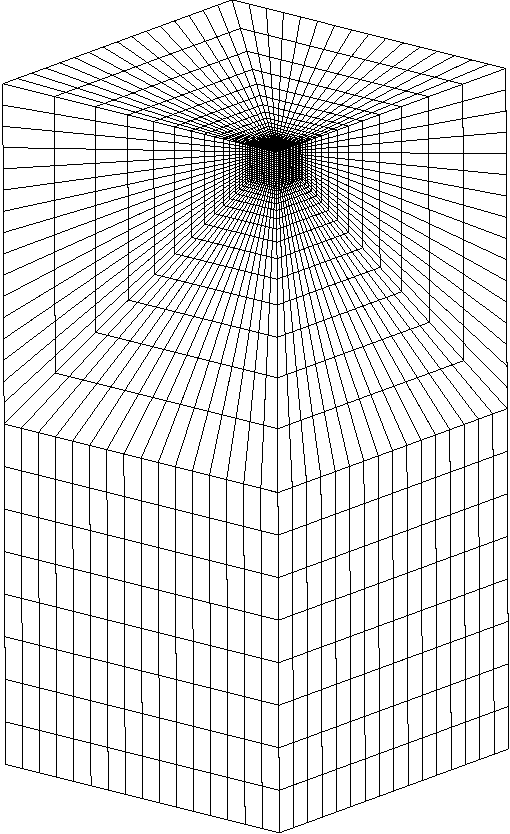
\includegraphics[height=0.30\textheight]{pictures/grid.png}
	\caption{Геометрия задачи и сетка.}
	\label{fig:grid}
\end{figure}
%\begin{figure}[h!]
%	\centering
%	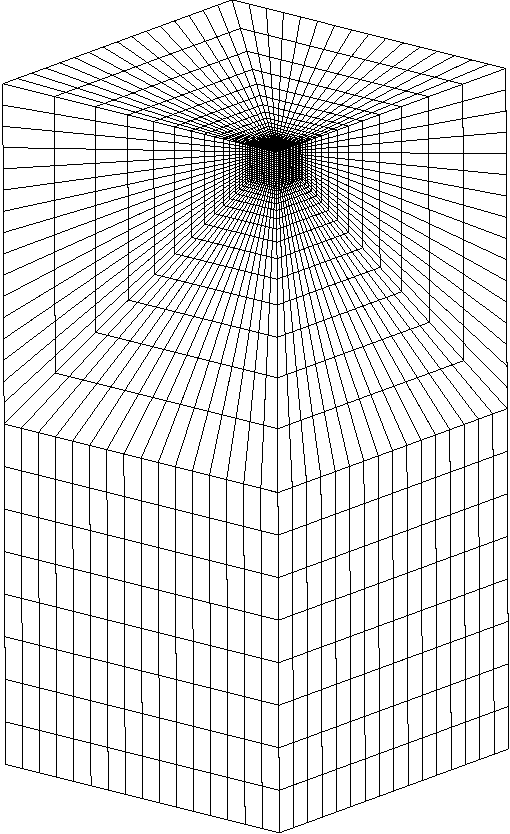
\includegraphics[height=0.30\textheight]{pictures/grid.png}
%	\caption{Сетка в сечении $y=0$ при $n=0$, $\bar{\delta}_{max}=110$, $\frac{E^*}{Y}=550$, $N=12$}
%	\label{fig:grid}
%\end{figure}

Общую силу реакции опоры $P$, глубину индентации $\delta$ (величину сближения удалённых точек) и площадь контактной поверхности $A$ можно представить в безразмерном виде \cite{Song2014}:
\begin{equation}
\begin{gathered}
\bar{P}=P/P_Y,\\
\bar{A}=A/A_Y,\\
\bar{\delta}=\delta/\delta_Y,
\label{F:test1_dimensionless_form1}
\end{gathered}
\end{equation}
где $P_Y$, $A_Y$, $\delta_Y$ --- значения, при которых начинается пластическое течение:
\begin{equation}
\begin{gathered}
P_Y=\frac{9\pi^3}{16} c^3 Y R^2\left(\frac{E^*}{Y}\right)^{-2},\\
A_Y=\frac{9\pi^3}{16} c^2 R^2\left(\frac{E^*}{Y}\right)^{-2},\\
\delta_Y=\frac{9\pi^2}{16} c^3 Y R\left(\frac{E^*}{Y}\right)^{-2}
\label{F:test1_dimensionless_form2}
\end{gathered}
\end{equation}
\begin{equation}
c=1.08,
\label{F:test1_dimensionless_form3}
\end{equation}
\begin{equation}
E^*=\frac{E}{1-\nu^2},
\label{F:test1_dimensionless_form4}
\end{equation}
$c$ --- константа для случая критерия пластического течения Мизеса, $E^*$ --- приведённый модуль упругости, $R$ --- радиус шара, $E$ --- модуль упругости полупространства, $\nu$ --- коэффициент Пуассона полупространства, $Y$ --- предел текучести полупространства.

Материал с изотропным степенным упрочнением задаётся диаграммой одноосного растяжения вида
\begin{equation}
\begin{cases}
\sigma=F\left(\varepsilon\right)\equiv E\varepsilon,\mbox{ если }\sigma<Y,\\
\sigma=F\left(\varepsilon\right)\equiv Y\left(\frac{\varepsilon}{\varepsilon_Y}\right)^n,\mbox{ если }\sigma\geqslant Y,
\end{cases}
\label{F:test1_isotropic_strain_hardening1}
\end{equation}
где $\varepsilon_Y=Y/E$, $Y$ --- предел упругости. Соответствующая функция $\sigma_y=\Phi\left(q\right)$ (см. \eqref{F:F_Flow2}) строится из соотношений
\begin{equation}
\Phi\left(q\right)=F\left(\varepsilon\right),\; \varepsilon-\frac{1}{E} F\left(\varepsilon\right)=q,
\label{F:test1_isotropic_strain_hardening2}
\end{equation}
т.к. $q\equiv\int d\tilde{\varepsilon}^{p}$ и в одноосном случае $\tilde{\sigma}=\sigma$, $d\tilde{\varepsilon}^{p}=d\varepsilon^{p}$. На рисунке \ref{fig:curves} приведены кривые для материала при различных \mbox{коэффициентах $n$}.

\begin{figure}[h!]
	\centering
	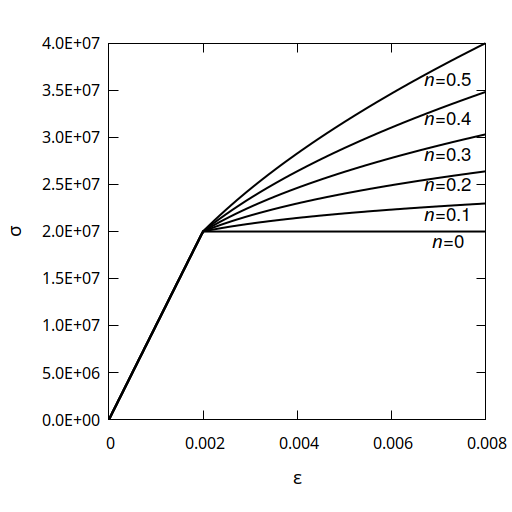
\includegraphics[height=0.25\textheight]{pictures/curves_diagr.png}
	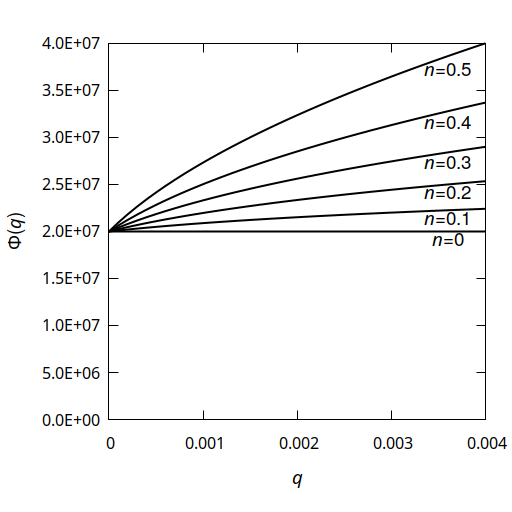
\includegraphics[height=0.25\textheight]{pictures/curves_f.png}
	\caption{ Диаграммы одноосного деформирования (слева) и соответствующие функции $\sigma_y=\Phi\left(q\right)$ (справа) для изотропного степенного упрочнения при ${\bar{\delta}_{max}=110}$, ${\frac{E^*}{Y}=550}$ и различных значениях коэффициента $n$.
	}
	\label{fig:curves}
\end{figure}

Параметры задачи приведены в таблице \ref{tab:test1_parameters}. Симметрия относительно плоскостей $x=0$ и $y=0$ учитывается однородными кинематическими краевыми условиями, и рассматривается $1/4$ образца. Сетка четвертинки изображена на \mbox{рисунке \ref{fig:grid}}. Размеры куба $H^{in}$, в котором наиболее подробная сетка, выбирались так, чтобы зона контакта не выходила за пределы его поверхности. Размеры куба $H^{out}$ выбирались в 10 раз больше, чем размеры $H^{in}$ (исходя из принципа Сен Венана). Коэффициент разрядки выбирался таким, чтобы примыкающие к граням $H^{in}$ конечные элементы были примерно одинакового размера. Были использованы базисные функции Лагранжа, первого порядка.

%\captionsetup[table]{singlelinecheck=off}

\begin{table}[h!]
	\caption{Параметры задачи}
	%\ctable [doinside=\small]
	
	%\begin{tabular}{|p{5.3cm}|c|p{7cm}|}
	%	\hline
	%	Параметр      & Обозначение & Значение  \\
	%	\hline
	\begin{tabular}{|p{5.3cm}|c|p{7cm}|}
		
		\hline
		Параметр & Обозначение & Значение \\
		\hline
		Модуль Юнга & $E$ & $10^{10}$ Па \\
		\hline
		Коэффициент Пуассона & $\nu$ & $0.3$ \\
		\hline
		Коэффициент степенного упрочнения& $n$ & $0, 0.1, ..., 0.9$ \\
		\hline
		Безразмерная глубина индентации&
		$\bar{\delta}_{max}$
		& $1,3,6,10,15,20,30,50,70,90,110$   \\
		\hline
		& $\frac{E^*}{Y}$ & $110, 220, 550, 1100$    \\
		\hline
		Радиус шара & $R$ & $1$м \\
		\hline
		Глубина индентации & $\delta$ & $\bar{\delta}_{max}\delta_Y$ \\
		\hline
		Размеры $H^{in}$ & $H_x^{in}\times H_y^{in}\times H_z^{in}$ & $H_x^{in}=H_y^{in}=H_z^{in}=1.5\sqrt{2R\delta-\delta^2}$\\
		\hline
		Размеры $H^{out}$ & $H_x^{out}\times H_y^{out}\times H_z^{out}$ & $H_x^{out}=H_y^{out}=H_z^{out}=10 H_x^{in}$\\
		\hline
		Разбиение $H^{in}$ & $N\times N\times N$ & $N=16$ \\
		\hline
		Коэффициент сгущения& $q$ & находится из решения уравнения  $\frac{1-q^{N-1}}{1-q^{N}}=\frac{H_x^{out}-H_x^{in}}{H_x^{out}}$ \\
		% \newline
		\hline
		Количество КЭ &  & $18432$ \\
		\hline
		Количество шагов нагружения/разгрузки &  & $110$ \\
		\hline
		Параметры завершения итераций & $\Delta_{\sigma}$, $\Delta_{\varepsilon}$, $\Delta_{F}$, $\Delta_{r}$ & $\Delta_{\sigma}=\Delta_{\varepsilon}=\Delta_{F}=10^{-10}$, \newline $\Delta_{r}=10^{-14}$ \\
		\hline
		Коэффициент в \eqref{F:F_algoritm_kappa} & $\omega^{c}$ & $10$ \\
		\hline
		Коэффициент в \eqref{F:F_algoritm_ep_new_active}& $\omega^{p}$ & $1$ \\
		\hline
		Коэффициент в \eqref{F:F_algoritm_unload_criterion2} & $cos\left(\theta_{\mathrm{min}}\right)$ & $0.1$ \\
		\hline
	\end{tabular}
	\label{tab:test1_parameters}
\end{table}

На рисунках \mbox{\ref{fig:res1}, \ref{fig:res2}, \ref{fig:res3}} приведены решения при различных параметрах задачи, полученные с помощью реализации приведённого в статье алгоритма; решения ANSYS, полученные на точно такой же сетке, с учётом больших деформаций; и численное решение аналогичной задачи в осесимметричной (двумерной) постановке из \cite{Song2014}. При решении в ANSYS без учёта больших деформаций значения $\bar{P}$ и $\bar{A}$ значительно отличаются от приведённых на рисунке \ref{fig:res1}, но остаточная глубина индентации $\bar{\delta}_{res}$ отличается не значительно.

\begin{figure}[h!]
	\centering
	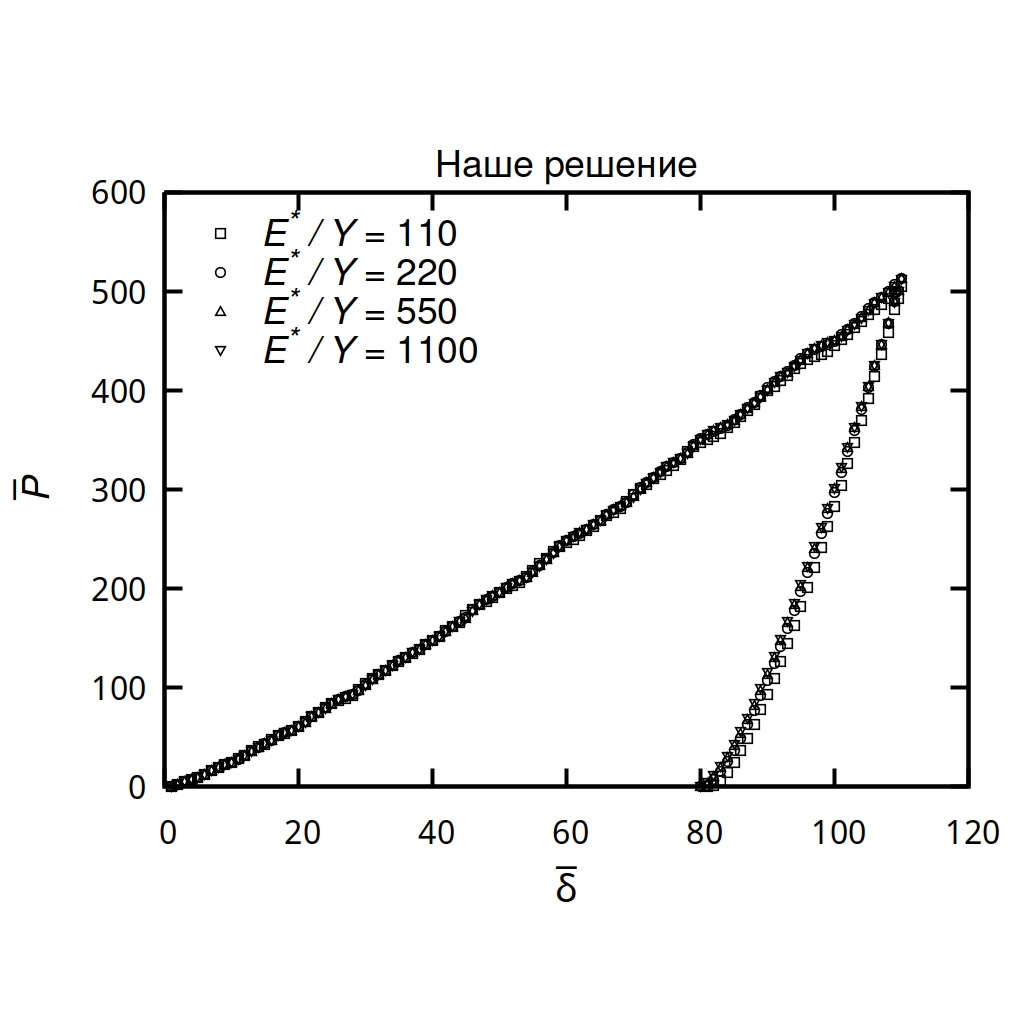
\includegraphics[height=0.25\textheight]{pictures/bP_bd.png}
	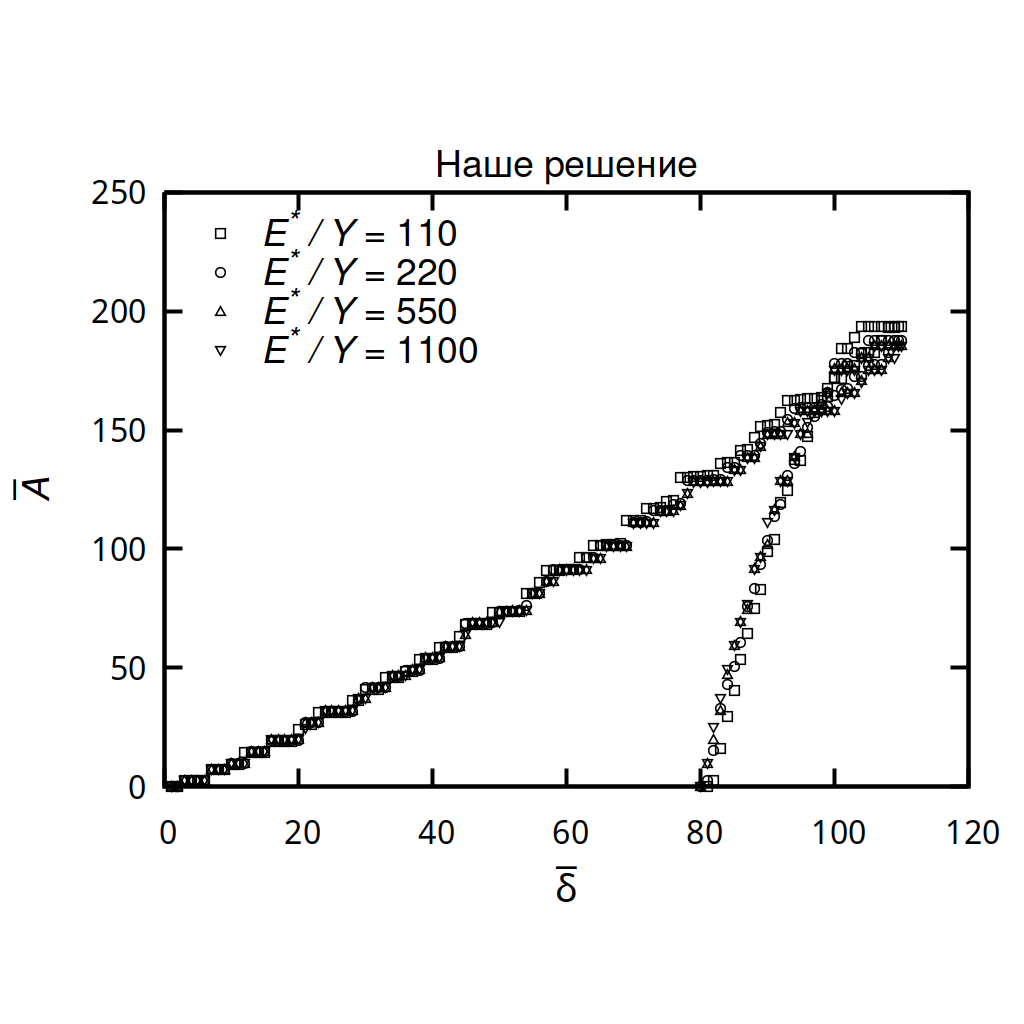
\includegraphics[height=0.25\textheight]{pictures/bA_bd_low.png}
	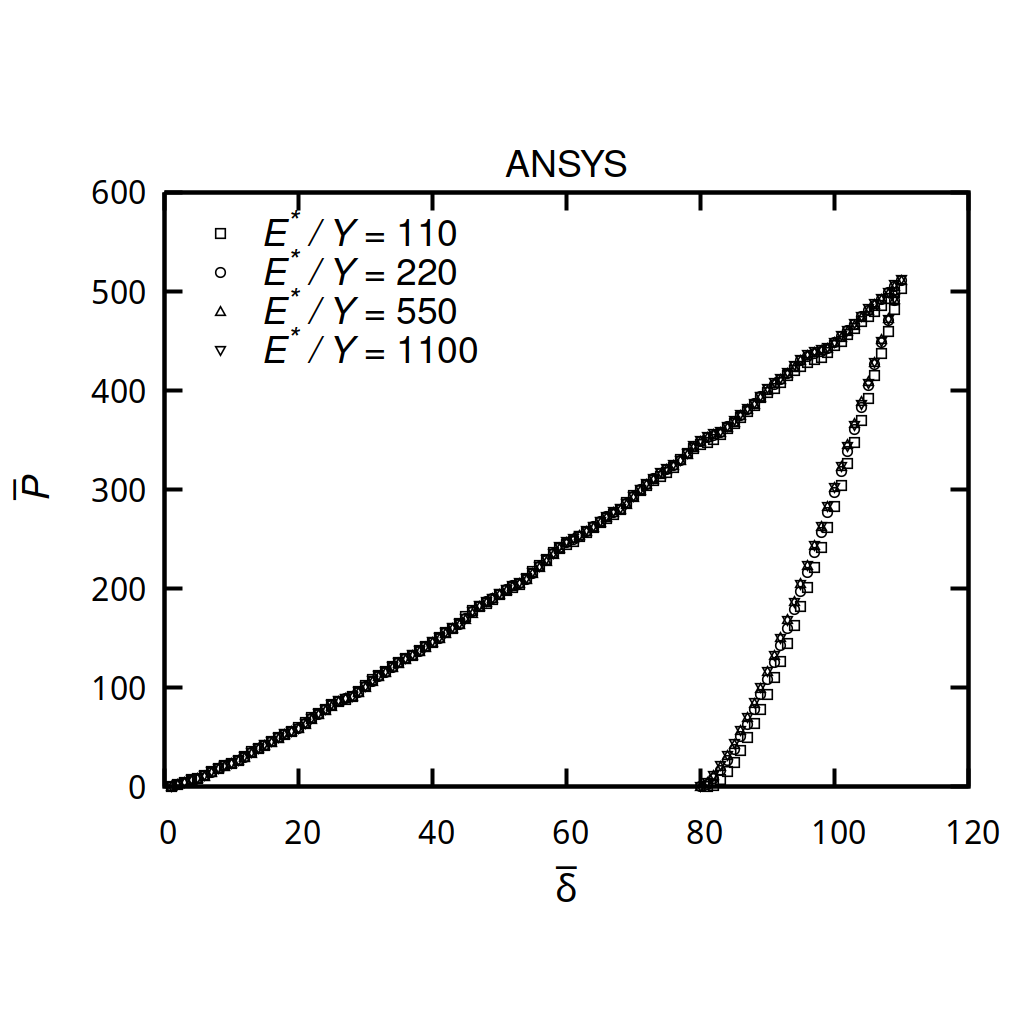
\includegraphics[height=0.25\textheight]{pictures/ANSYS_bP_bd.png}
	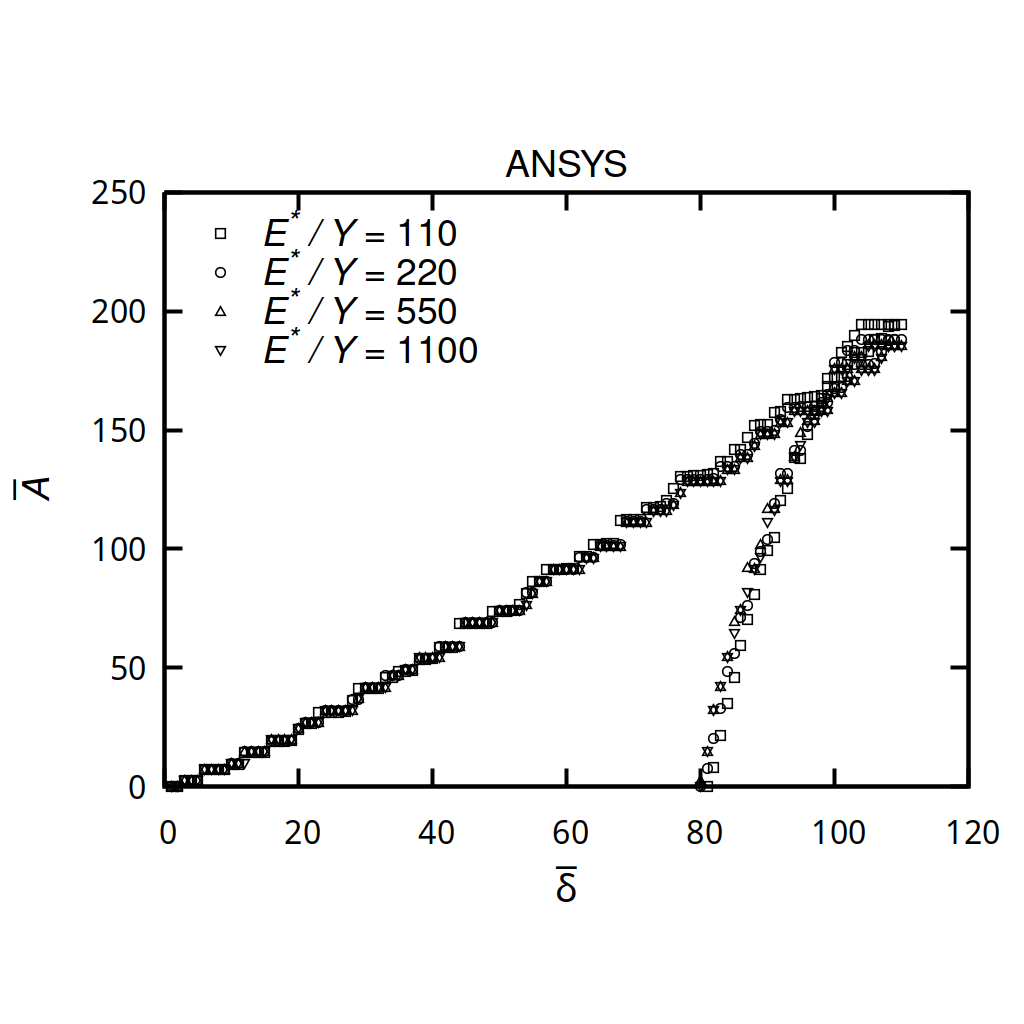
\includegraphics[height=0.25\textheight]{pictures/ANSYS_bA_bd_low.png}
	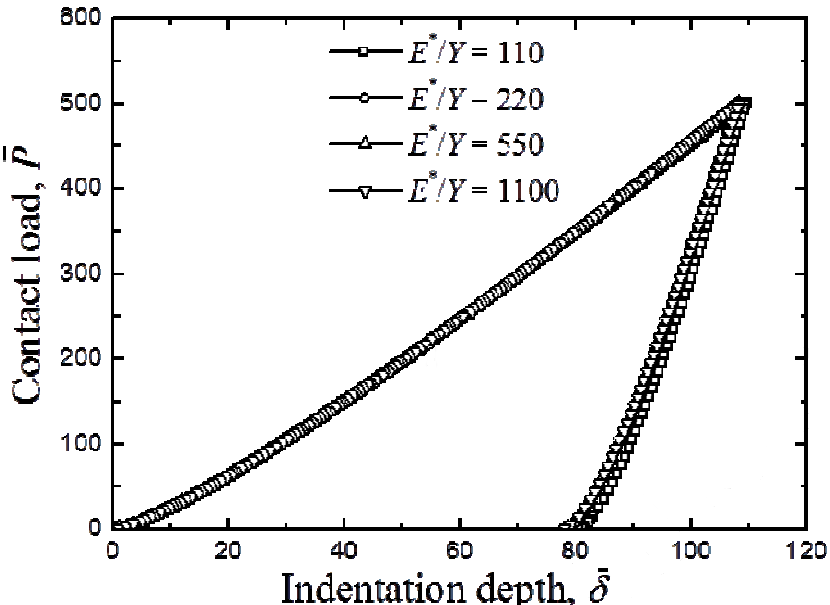
\includegraphics[height=0.18\textheight]{pictures/F2_a.png}
	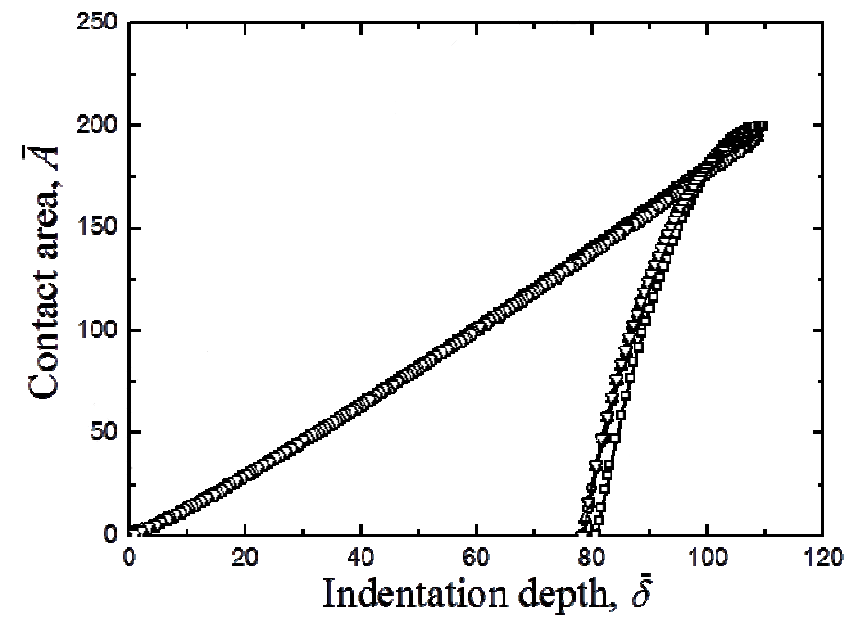
\includegraphics[height=0.18\textheight]{pictures/F2_b.png}
	\caption{ Зависимости общей силы реакции опоры $\bar{P}$ (слева) и площади контактной поверхности $\bar{A}$ (справа) от глубины индентации $\bar{\delta}$ при ${n=0}$, ${\bar{\delta}_{max}=110}$, ${\frac{E^*}{Y}=110, 220, 550, 1100}$. Сверху полученное численное решение, по середине решение ANSYS, снизу численное решение из \cite{Song2014}.
	}
	\label{fig:res1}
\end{figure}
\begin{figure}[h!]
	\centering
	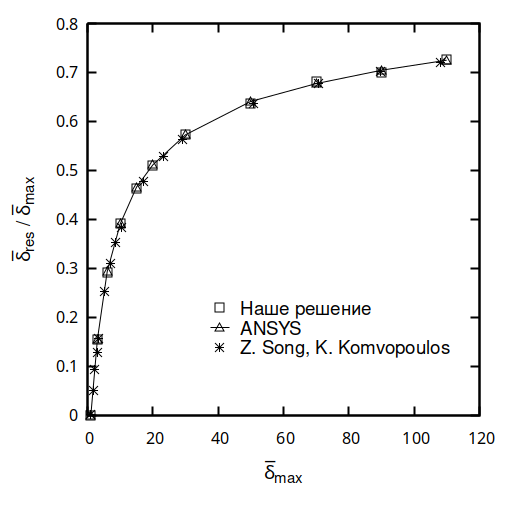
\includegraphics[height=0.25\textheight]{pictures/bd_residual_bd_max.png}
	\caption{Зависимость остаточной глубины индентации $\bar{\delta}_{res}$ (по отношению к $\bar{\delta}_{max}$) от максимальной глубины индентации при ${n=0}$, ${\bar{\delta}_{max}=1,3,6,10,15,20,30,50,70,90,110}$, ${\frac{E^*}{Y}=550}$.
	}
	\label{fig:res2}
\end{figure}
\begin{figure}[h!]
	\centering
	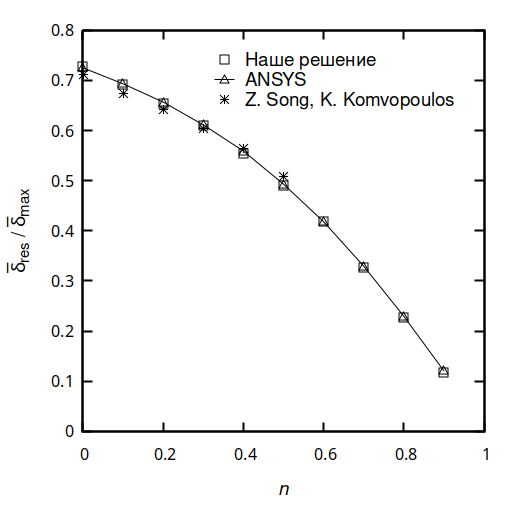
\includegraphics[height=0.25\textheight]{pictures/bd_residual_n.png}
	\caption{ Зависимость остаточной глубины индентации $\bar{\delta}_{res}$ (по отношению к $\bar{\delta}_{max}$) от коэффициента степенного упрочнения при ${n=0, 0.1, ..., 0.9}$, ${\bar{\delta}_{max}=110}$, ${\frac{E^*}{Y}=550}$.
	}
	\label{fig:res3}
\end{figure}

Значения $\bar{A}$, $\bar{P}$ и $\bar{\delta}_{res}$ в нашей реализации и в ANSYS вычислялись одинаковыми способами. Площадь получена путём суммирования площадей 4-угольных граней конечных элементов, все 4 узла которых находятся в состоянии контакта, т.е. рассчитывалась нижняя оценка площади. Общая сила реакции опоры вычислялась суммированием сил в контактных узлах. Остаточной глубиной считалась глубина индентации на шаге, на котором полностью пропадает контакт.

На рисунке \ref{fig:iterations} приведены характеристики итерационного процесса для нескольких параметров задачи. Количество изменений матрицы СЛАУ в результате разгрузок на КЭ (физических или численных из-за наличия вектора узловых невязок $\mathbf{R}^{\mathrm{node}}$ или погрешности) лишь на некоторых шагах превосходит 2, количество итераций на каждом шаге \mbox{меньше 40}. 

\begin{figure}[h!]
	\centering
	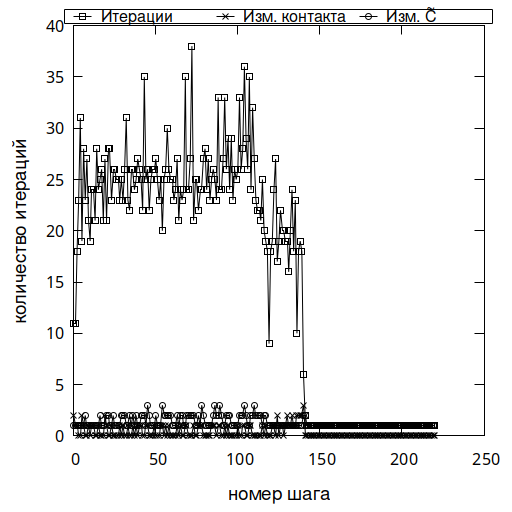
\includegraphics[height=0.22\textheight]{pictures/I_0550.png}
	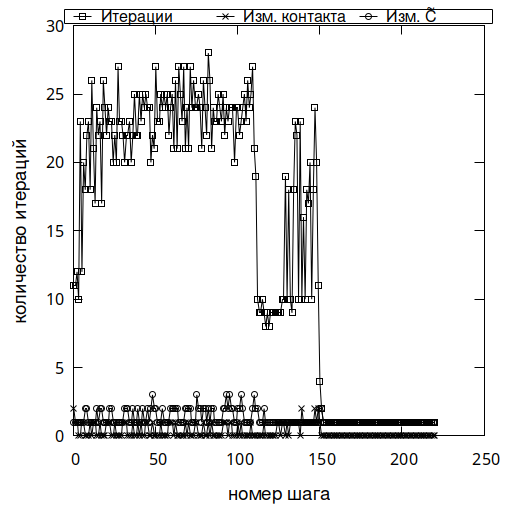
\includegraphics[height=0.22\textheight]{pictures/II_050.png}
	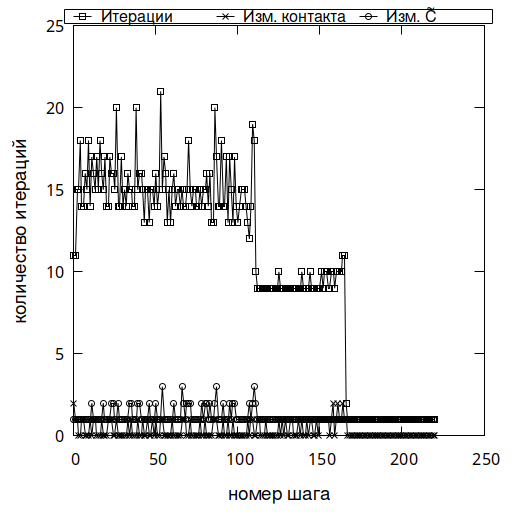
\includegraphics[height=0.22\textheight]{pictures/III_0.5.png}
	\caption{ Количество итераций и изменений матрицы из-за разгрузки или изменения статусов контактных узлов при ${n=0}$, ${\bar{\delta}_{max}=110}$, ${\frac{E^*}{Y}=550}$ (слева), ${n=0}$, ${\bar{\delta}_{max}=50}$, ${\frac{E^*}{Y}=550}$ (по середине) и ${n=0.5}$, ${\bar{\delta}_{max}=110}$, ${\frac{E^*}{Y}=550}$ (справа).
	}
	\label{fig:iterations}
\end{figure}



\section{Заключение}
Проверка реализации приведённого алгоритма на модельной задаче показала удовлетворительные результаты, не смотря на неизменность при итерациях значений направляющих тензоров $z\equiv\frac{\partial{}^{(t)}\tilde{\sigma}}{\partial\sigma}$ и $\frac{{}^{(t)}s}{{}^{(t)}\tilde{s}}$. В случае быстрого поворота траектории сложного нагружения, для лучшей сходимости можно обновлять эти значения (или только одно), например, по правилу трапеций или средней точки \cite{Ortiz1985} и вместо непрерывного (continuum) упругопластического тензора \eqref{F:F_alg_C_pl} использовать согласованный (consistent) с алгоритмом возврата на поверхность текучести \cite{Simo1985} или \cite{Gu2011} и т.п. Для простоты, мы эти модификации здесь рассматривали. Нормаль к поверхности штампа $\mathbf{n}=Norm\left({}^{(t)}\mathbf{x}\right)$ так же можно обновлять после каждой итерации, и дополнительные вычислительные затраты на разложения матрицы будут не значительными, если степени свободы контактных узлов (которых на поверхности не много) хранить в нижней части матрицы СЛАУ.
 
%\clearpage
% библиография
\begin{thebibliography}{3}
\bibitem{Bathe1982}
Bathe K.-J. Finite Element Procedures in Engineering Analysis. En-glewood Cliffs, New York: Prentice-Hall, 1982.
\bibitem{Zienkiewicz1975}
Зенкевич О. Метод конечных элементов в технике. --- М. : Мир, 1975. --- 542 с.
\bibitem{Burago2005}
Бураго Н. Г., Кукуджанов В. Н. Обзор контактных алгоритмов //Известия Российской академии наук. Механика твердого тела, 2005. --- №. 1. --- С. 45-87.
\bibitem{Wriggers2006}
Wriggers P. Computational Contact Mechanics. --- Springer Science \& Business Media, 2006.
\bibitem{Pisarenko1981}
Писаренко Г. С., Можаровский Н. С. Уравнения и краевые задачи теории пластичности и ползучести. --- Киев : Наукова думка, 1981. --- 496 с.
\bibitem{Kravchuk1994}
Кравчук А. С. Вариационные и квазивариационные неравенства в механике. --- РФФИ, 1994. --- 334 с.
\bibitem{Korobeynikov2000}
Коробейников С. Н. Нелинейное деформирование твердых тел. --- Новосибирск : Издательство СО РАН, 2000. --- 262 с.
\bibitem{SoloveychikRoyakPersova2007}
Соловейчик Ю. Г., Рояк М. Э., Персова М. Г. Метод конечных элементов для решения скалярных и векторных задач. --- Новосибирск : Изд-­во НГТУ, 2007. --- 895 с.
\bibitem{Frolov1995}
Александров А. В., Алфутов Н. А., Астанин В. В. и др. Энциклопедия ”Машиностроение”. Том I-­3. ”Динамика и прочность машин. Теория механизмов и машин”. В 2-­х книгах. Кн. 2 / Под ред. Фролов К. В. (гл. ред.). --- М. : Машиностроение, 1995. --- 624 с.
\bibitem{Belytschko2000}
Belytschko T., Liu W. K., Moran B. Nonlinear finite elements for continua and structures, 2000.
%\bibitem{OtchetPNI}
%Отчет о ПНИ по теме: "Разработка программно-технических решений в области промышленного программного обеспечения для моделирования поведения элементов конструкций из современных материалов в экстремальных условиях при механических и немеханических воздействиях для решения задач проектирования авиакосмической техники" (No гос. регистрации: 114112440083)
\bibitem{Johnson1989}
Джонсон К. Механика контактного взаимодействия : пер. с англ. --- М. : Мир, 1989.
\bibitem{Song2014}
Song Z., Komvopoulos K. An elastic–plastic analysis of spherical inden­tation: Constitutive equations for single­indentation unloading and development of plasticity due to repeated indentation // Mechanics of Materials, 2014.
\bibitem{Ortiz1985}
Ortiz M., Popov E. P. Accuracy and stability of integration algorithms for elastoplastic constitutive relations //International journal for numerical methods in engineering. – 1985. – Т. 21. – №. 9. – С. 1561-1576.
\bibitem{Simo1985}
Simo J. C., Taylor R. L. Consistent tangent operators for rate-independent elastoplasticity //Computer methods in applied mechanics and engineering, 1985. --- Т. 48. --- №. 1. --- С. 101-118.
\bibitem{Gu2011}
Gu Q. et al. Consistent tangent moduli for multi-yield-surface $J_2$ plasticity model //Computational Mechanics, 2011. --- Т. 48. --- №. 1. --- С. 97-120.
\end{thebibliography}













\end{document}
